% -*- root: diplomarbeit.tex -*-
\section{Auswertung und Ausblick}
	Object Detection ist eines der herausfordernsten Forschungsfelder in Computer Vision. Obwohl die Entwicklung von robusten und gut funktionierenden Ansätzen in den letzten Jahren stark zugenommen hat und unter kontrollierten Bedingungen auch sehr gute Ergebnisse liefert, ist das Problem des Suchens und Findens von einem oder mehreren Objekten in der ``realen'' Welt weiterhin ungelöst \cite{ODS}.

\subsection{Evaluation}
	Die Evaluation von TLD erfolgt mit Hilfe eine Standardverfahrens zur Beurteilung von Klassifikatoren und findet auch in \cite{TLD} Verwendung. Hierbei dienen die quantitativen Ergebnisse des Klassifizierers in jedem Testszenario als Maß. Da TLD ein binärer Klassifizierer ist, gibt es zwei Arten von Fehlern die auftreten können. Entweder wird das Objekt in die Klasse $A$ eingeordnet, obwohl es zu $B$ gehört, oder es wird als Teil von $B$ bestimmt, gehört allerdings zur Klasse $A$. $A$ und $B$ sind in Falle von TLD ``gefunden'' und ``nicht gefunden''.

	Als Vergleichsbasis dient der Ground Truth. Das ist der Bereich, der die genaue Position des gesuchten Kopters im Bild markiert, gegeben durch eine BoundingBox $BB_{GT}$. Dieser wird mit dem Ergebnis von TLD verglichen, der ebenfalls eine BoundingBox $BB_{TLD}$ bei erfolgreicher Detektion beziehungsweise erfolgreichem Tracking liefert. Zwischen beiden Boxen wird die Überlappung bestimmt und geprüft, ob sie größer oder kleiner eines Thresholds $\omega$ ist. Daraus ergeben sich vier Fälle:

	\begin{description}
		\item [True-Positive $t_p$] Die Überlappung ist größer als $\omega$.
		\item [True-Negative $t_n$] Es wurde kein Objekt gefunden und es wurde auch keines erwartet.
		\item [False-Positive $f_p$] Der Algorithmus findet ein Objekt, obwohl keines erwartet wurde, oder die Überlappung ist kleiner als $\omega$.
		\item [False-Negative $f_n$] Der Algorithmus findet kein Objekt, obwohl eines erwartet wurde, oder die Überlappung ist kleiner als $\omega$.
	\end{description}

	In jedem Testdurchlauf werden die Anzahl $t_p$, $t_n$, $f_p$ und $f_n$ gezählt und mittels statistischer Gütekriterien ausgewertet.
  Wie auch bei \cite{TLD} sind diese Kriterien Genauigkeit (Precision) \begin{equation} P=\frac{t_p}{(t_p + f_p)},\end{equation}
  Trefferquote (Recall) \begin{equation} R=\frac{t_p}{(t_p + f_n)} \end{equation}
  und das gewichtete harmonische Mittel \begin{equation} F=\frac{2 \times (P \times R)}{(P + R)}.\end{equation}

\subsection{Resultate}
	Hier kommen die Resultate der Testreihen

\subsection{Auswertungen und Beobachtungen}
	\label{subsec:conclusion}
	TLD beeindruckt durch sehr gute Ergebnisse beim Tracken von unterschiedlichen und unbekannte Objekten, wie Fußgänger, Autos und Gesichtern \cite{TLD}. Als Detektionsstrategie ist dieser semi-supervised-learning-Ansatz für eine Vielzahl von Fällen geeignet. Die natürlich gegebenen Umwelteinflüsse wie zum Beispiel unterschiedliche Beleuchtungen der Szenerie durch Licht-Schatten-Wechsel werden durch die Detektorkaskade gut verarbeitet. Wie die Resultate jedoch verdeutlichen, ist TLD trotz der vielen Stärken für die Koptererkennung nur bedingt leistungsfähig. Die Gründe werden im Folgenden vorgestellt und analysiert.

	\paragraph{Detektorkaskade}
	Die letzte Komponente der Detektorkaskade, der NearestNeighbour Classifier, speichert Patches des Objekts in der Größe $15\times15 px$. Bestimmt durch die BoundingBox wird meist auch ein Teil des Hintergrundes gespeichert und gelernt. Somit ist nicht nur das Objekt selbst, sondern auch seine Umgebung Teil der Repräsentation. Der Einfluss ist hierbei stark von Größe und Beschaffenheit des Objekts sowie der Menge an ``Hintergrund'', der gespeichert wird, abhängig.

	Ein Kopter wird durch einen anderen Kopter meist von der Seite wahrgenommen. Aufgrund der filigranen Struktur wird unweigerlich immer eine Menge Hintergrundinformationen im Patch gespeichert. Der Einfluss auf die Genauigkeit und die Trefferquote des Detektors ist damit sehr groß. Probleme treten vor allem dann auf, wenn der Hintergrund einen hohen Informationsgehalt hat, wie zum Beispiel Bäume oder Häuser, da der Kopter selbst strukturell eher einfach aufgebaut ist. Aber auch Hintergründe mit unterschiedlichen Farbstärke sind problematisch. So kann es vorkommen, dass ein Kopter, dessen Model vor einem hellen Hintergrund ``erlernt'' wurde, vor einem dunklen nicht mehr erkannt wird.

	\paragraph{MedianFlow Tracker}
	Die Struktur des Kopters bedingt nicht nur den Erfolg des Detektors, sondern beeinflusst ebenfalls die Leistung des Trackers. Dieser schätzt anhand einer regelmäßigen Anordnung von Punkte innerhalb einer BoundingBox in einem Bild die Position der Punkte im Folgebild. Diese regelmäßige Anordnung ist gleichförmig, wodurch viele Punkte, die zum Hintergrund gehören, die LKT-Schätzung beeinflussen (Abbildung \ref{abb:problem_tracker}). Auch hier stellen vor allem detailreiche Hintergründe ein Problem dar, weil durch die willkürliche Wahl der Punkte die Wahrscheinlichkeit erhöht wird, eine ungenaue Schätzung zu erhalten.

	Ein zusätzlicher Nachteil des Trackers ist, dass er keine Lernkomponente besitzt. Jede Verarbeitung ist unabhängig und integriert keine zusätzlichen Informationen aus vergangenen Schätzungen, was bedeutet, dass der Tracker immer wieder die gleichen Fehler macht - im Gegensatz zum Detektor, der aus seinen Fehlern ``lernt'' und versucht.

	Abbildung \ref{abb:problem_background_1} verdeutlicht die angesprochenen Fehler. Während in (a) die Berechnung der Trajektorie noch fehlerfrei funktioniert, wird in (b) deutlich, dass der Hintergrund fälschlicherweise als Teil des Objekts erkannt wird. An dieser Stelle sollte der Tracker reinitialisiert werden, weil die Bewertung der Tracker-Box einen schlechten $conf-$Wert ergibt. Problematisch wird es jedoch, wenn das Model des Objekts zu diesem Zeitpunkt unzureichend gelernt wurde. Damit kann es vorkommen, dass Bewertung der Detektor-Box weiterhin schlechter ist, als die des Trackingergebnisses. In (c) wird dadurch das Objekt nicht mehr fokussiert und die Trajektorie falsch geschätzt. Zusätzlich werden fälschlicherweise neue Objektrepräsentationen generiert, weil TLD den eigenen Fehler nicht erkennt. Als Folge wird das Model verfälscht.

	\begin{figure}[H]
		\begin{centering}
			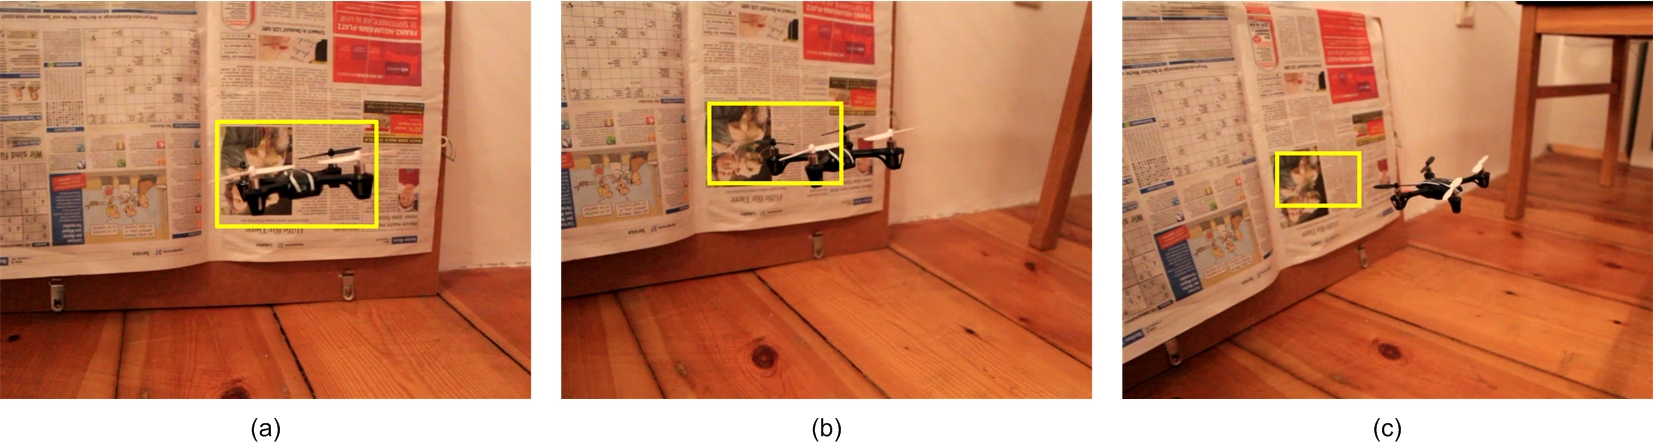
\includegraphics[scale=0.5]{../pictures/problem_background_1.jpg}
			\caption{Trackingprobleme bei zu hoher Informationsdichte des Hintergrunds.}
			\label{abb:problem_background_1}
			\par
		\end{centering}
	\end{figure}

	Um den Einfluss des Hintergrundes zu minimieren, ist es möglich nur einen Teil des Kopters initial zu markieren, wie zum Beispiel den Corpus ohne die Rotoren, wie in Abbildung \ref{abb:problem_background_2} dargestellt. Das führt allerdings dazu, dass der Kopter in (a) ausschließlich anhand dieses Teilbereichs erkannt wird. In (b), wenn sich die Positionen von Kamera und Kopter ändern, wird der markierte Bereich vom Kopter selbst verdeckt. In (c) ist der Teilbereich nicht mehr zu sehen und der Kopter wird nicht mehr erkannt. Das macht es unmöglich ein vollständiges Model des Objekts zu generieren.

	\begin{figure}[H]
		\begin{centering}
			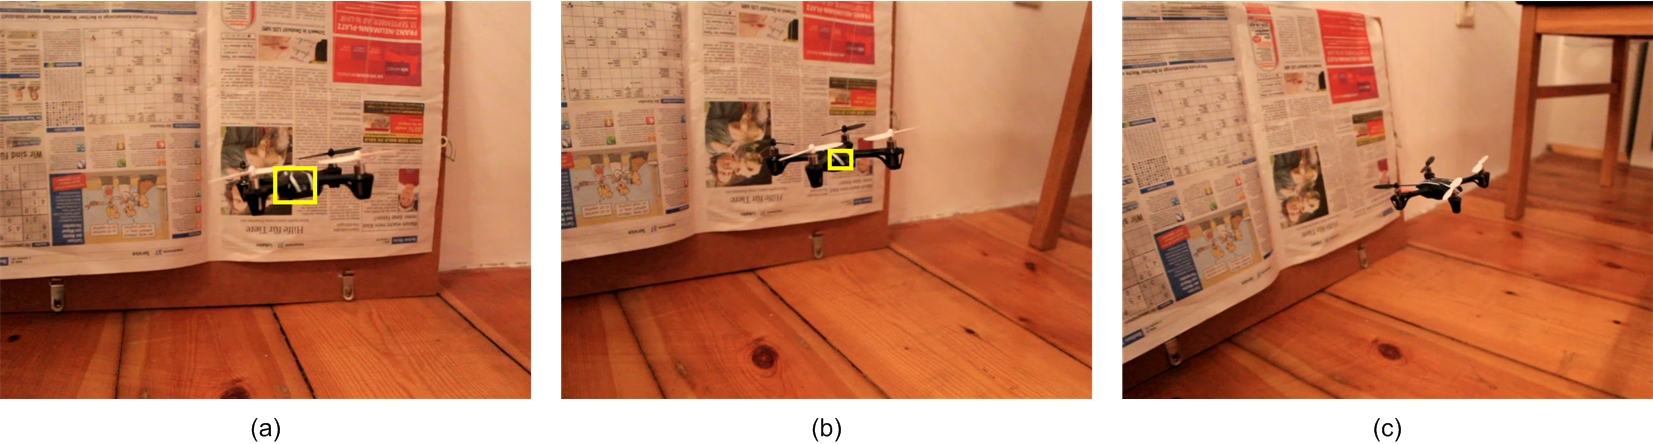
\includegraphics[scale=0.5]{../pictures/problem_background_2.jpg}
			\caption{Trackingprobleme bei Teilmarkierung des gesuchten Objekts.}
			\label{abb:problem_background_2}
			\par
		\end{centering}
	\end{figure}



	% Der Ansatz ist nur bedingt geeignet. Probleme:
	% \begin{itemize}
	% \item Speichern der Beispiele in Form von $15\times15$ patches, weil zu viel Hintergrund gespeichert wird,
	% \item Objekt (Kopter) hat filigrane Struktur,
	% \item ``Veschmelzung'' des Objekts mit dem Hintergrund
	% \end{itemize}
	% Weiteres...
	% \begin{itemize}
	% \item Ein paar Worte zur Umsetzung (openCV)
	% \item Erweiterungsmöglichkeiten - z.B. Verfolgung mehrerer Kopter gleichzeitig, Optimierungsvorschläge, weitere Einsatzmöglichkeiten (da TLD an sich ``alles'' tracken kann)
	% \item Zusammenfassung
	% \item ohne zusätzlich Detectionsverfahren (eventuell Tiefenbilder oder andere nicht-visuelle Ansätze) kaum möglich
	% \item Umwelteinflüsse in der Natur sind zu stark
	% \item Einfluss der unterschiedlichen Beleuchtungen der Szene
	% \item Hintergrund (Bäume etc)
	% \item Problem bei zusätzlichen Verfahren: Rechenleistung des Roboters(?)
	% \end{itemize}

\subsection{Modifikationen und Verbesserungsvorschläge}
	Die strickte Trennung der einzelnen Komponenten in TLD bietet die Möglichkeit eine Reihe von Änderungen vorzunehmen, ohne die prinzipielle Arbeitsweise zu verändern. Das ist eine zusätzliche Stärke des Algorithmus. Im folgenden Abschnitt werden Modifikationen diskutiert, die TLD für die Koptererkennung leistungsfähiger machen können.

	\paragraph{Detectorkaskade}
		Neben der in \cite{TLD} diskutierten Vorschläge, wie zum Beispiel einen Forground Filter, der allerdings in dieser Arbeit sicherlich signifikanten Verbesserungen nach sich ziehen würde, weshalb auf eine Implementation verzichtet wird, gibt es weitere Anpassungen der Detektor-Komponente, die hier diskutiert werden.

		Wie in \ref{subsec:conclusion} erläutert, ist die Datenbasis des NearestNeigbour Classifier für die Koptererkennung ungeeignet. Die Struktur des Objekts bedingt das Speichern von zu vielen Hintergrundinformationen, was die Berechnung des $conf$-Wertes und damit die Klassifikation stark negativ beeinflusst. Ein andere Repräsentation, eventuell mit herausgefiltertem Hintergrund oder einer anderen Speicherform als Patch wäre sinnvoll.

	\paragraph{MedianFlow Tracker}
		Zum einen könnte die Tracker-Komponente mit einem anderen Verfahren die Punkte für die Schätzung wählen. Eventuell würde eine nicht gleichförmige Verteilung der Punkte innerhalb der BoundingBox die Genauigkeit erhöhen und die Fehleranfälligkeit verringern. Eine Verringerung der Punktedichte vom Zentrum aus zu den Rändern der Box könnte den Einfluss des Hintergrunds auf das Ergebnis verringert.

		Das Ersetzen der MedianFlow Trackers durch eine andere Komponente wäre ebenfalls möglich. Trackingimplementationen mittels {\em Kalman-Filter} \cite{KAF} oder {\em Particle-Filter} \cite{PAF} liefern sehr gute Ergebnisse. Anstelle der Punktrepräsentation wären eine Objektdefinition anhand der Form oder signifikanter Linien denkbar und wurden auch bereits erfolgreich eingesetzt \cite{AVT}.

		Neben dem Ersetzen des MedianFlow Trackers könnte ein vollkommener Verzicht in Frage kommen, da er die fehleranfälligste Komponente in TLD ist. Das bedeutet allerdings, dass das Model des Objekts in vorherige Lernphasen offline gelernt werden muss. Die Strategie wäre somit die Klassifizierer in verschiedenen Szenarien intensiv zu trainieren und das Koptermodel in möglichst vielen Situationen zu lernen. Dies kann mittels TLD geschehen und wurde auch während der Testphasen in \ref{subsection:learning_and_testing} entsprechend durchgeführt. Im Anschluss wird der MedianFlow Tracker und damit auch die Lernkomponente deaktiviert. Also positive Folge kann das erlernte Model durch fehlerhafte Beispiele nicht länger verfälscht werden und die Laufzeit wäre optimiert, da durch fehlende Lernphasen und das Tracking Ressourcen gespart werden können. Negativ ist jedoch die fehlende Anpassung an neue Situation, was im Grunde eine der Stärken von TLD ist.

	\paragraph{Allgemein}
		Der Kopter soll selbst sein bestes Modell darstellen, weshalb als Vorgabe gilt, dass keine Modifikationen an ihm vorgenommen werden sollen. Dazu gehören Markierungen jeglicher Art, wie zum Beispiel Farb- oder Musterapplikationen. Deshalb wurde TLD für die Implementation gewählt, weil die Verarbeitung grundsätzlich mit jedem Objekttyp funktioniert und keine speziellen Modifikationen am Objekt nötig sind. Wie die Resultate und die Auswertung zeigen, ist diese Restriktion jedoch zu stark, denn der Kopter selbst ist nicht signifikant genug, um sich von seiner Umgebung ausreichend abzuheben. Die Verarbeitung zusätzlicher Informationen zur Verbesserung der Lösung ist anzuraten und wird kurz präsentiert.

		TLD arbeitet prinzipiell farbunabhängig, die Berechnung erfolgt einzig auf Grauwertbildern. Spezielle Markierungen auf den Flugrobotern könnten die Ergebnisse verbessern. Ähnlich der Szenarien beim \textit{Robocup}, wo eine signifikante Kombination eines horizontalen Streifenmusters zum Beispiel die Spielbegrenzung markiert, wären eine ähnliche Vorgehensweise bei der Markierung der Kopter denkbar. Wenn dieses Muster Teil der Objektrepräsentation ist, wird der Kopter signifikanter und hebt sich besser von seiner Umgebung ab.

		Eine Implementierung zur Verarbeitung von Farbbildern wäre ebenfalls eine Möglichkeit die Leistungsfähigkeit zu verbessern. Dazu müssen allerdings die im Allgemeinen uniformen Kopter farblich markiert werden, was wiederum den Restriktionen widerspricht.

% Verbesserungen/Ansätze
% \begin{itemize}
% \item eventuell stärke Orientierung an natürlich Seh-prozessen bzw. Sensoren in der Natur (Auge der Fliege)
% \item Eventuell ein anderer Ansatz: Vielleicht sollte man eine 3-D Repräsentation des Objekts während des Trackens erzeugen? Der Mensch macht es sicher auch nicht anders. Schließlich weiß man ja oft, wonach man suchen muss, auch wenn das Erscheinungsbild des Objekts nicht mit dem bereits ``Erlernten'' übereinstimmt...
% \item Articulated shape models > hierbei werden Teile des Objekts einzeln repräsentiert und zu einem ganzen Zusammengesetzt.
% \item Eventuell nicht so allgemeine Ansätze, sondern vorher viel mehr Wissen über das Objekt, den Kopter, als Grundlage nehmen. Eventuell ein 3- -Modell erzeugen und aus dem ermittelten Bild alle entsprechende Objekte auf dieses ``mappen''.
% \end{itemize}